\chapter{IMPLEMENTATION}

\section{IMPLEMENTATION GOALS} \label{sec:impgoals}
\paragraph{}
The goal of this implementation is to propose a real-time rendering technique that will render global illumination on the GPU through the use of OpenGL and GLSL.  We will use the idea of virtual point lights from \textit{Instant Radiosity} \cite{Keller1997} to render the indirect illumination.  Shadow maps will be used as in the spirit of \cite{Williams1978} and \cite{Reeves1987} to render shadows for direct illumination.  Shadow maps will also be used to render indirect shadows.  The VPL's will be structured outward from the primary light source in hemispheres using specific distances and angles around the primary light source. The goal is to simulate multiple waves of VPL's flowing outward from the primary light source in order to simulate the light transport as wave-like and therefore simulate indirect illumination using only the direct illumination of many VPL's while ignoring the bouncing of light among surfaces thus simplifying the Neumann series to just one term.  This way, we simulate light as a particle by using VPL's and as a wave in the way the VPL's will be organized.  This will allow the ``wrapping'' of light around objects in order to illuminate surfaces that may not be directly visible from the light source.  An additional goal of this implementation is to have the resulting technique be scalable.  The organization of the VPL's will allow us to use more or less VPL's depending on quality and performance desires along with additional parameters that will provide us with further balancing capabilities.  Specific implementation details will follow in section \ref{sec:impdetails}.  Lastly, in support of this technique and its ignorance of calculating true indirect illumination and instead using a direct illumination approximation of indirect illumination, we discuss the importance of using a scientifically correct rendering versus a visually appealing rendering.

\section{SCIENTIFICALLY CORRECT VERSUS VISUALLY APPEALING} \label{sec:study}
\paragraph{}
All of the previous work mentioned in chapter \ref{sec:prevwork} used approximations when computing indirect illumination to varying degrees.  This is because as mentioned in section \ref{sec:render}, the rendering equation (equation \ref{eqn:render}) is calculated using a Neumann series and in order to get an exact calculation, an infinite number of iterations would need to be carried out to fully calculate the result.  These iterations account for the infinite number of indirect light bounces that take place.  Since this is unfeasible, approximations are made based off our demands for performance or realism.  For real-time applications, we must err on the side of performance, but since the presence of indirect light has been shown to be perceptually important we can't just simply ignore it either \cite{Stokes2004}.  Also, according to \cite{Stokes2004}, diffuse indirect illumination is perceptually the most important component to consider.  However, as the notion of ``realism'' is merely whether the rendering is visually pleasing to the human eye, major approximations can be made to increase performance provided the result is visually pleasing.  As such, we ignore the bouncing of light and try to approximate it using only direct lighting that will be able to reach surfaces only visible to indirect light in order to simulate the ``feeling'' of indirect light.  Proof of the idea that visually pleasing is sufficient is provided next.

\paragraph{}
In \textit{Perceptual Influence of Approximate Visibility in Indirect Illumination} \cite{Yu2009} it is proven that ``accurate visibility is not required and that certain approximations may be introduced.''  When a person sees lighting rendered in a scene or in real-life, the most revealing or obvious lighting is the direct illumination.  When it is approximated or incorrect, it is apparent right away due to the high-frequency nature of direct lighting.  Indirect lighting, however is usually low-frequency and therefore has smooth graduations in changes of intensity.  This allows for more leeway for approximations and interpolations.  This is important since the most expensive calculation is the visibility determination for indirect shadows as will become apparent in the results section.  

\paragraph{}
To research the effects of this on the viewer's perception of the rendering, \cite{Yu2009} conducted a psychophysical study involving two different experiments.  The first experiment involved estimating the difference between the approximation rendering and the reference rendering using a number scale ranging from one to five corresponding to ``not similar'' and ``extremely similar'' respectively.  This experiment had 14 participants.  The second experiment involved ranking 10 approximated renderings and 1 reference rendering in order of least realistic to most realistic.  This experiment had 18 participants.  Over half of the participants in both experiments were computer  scientists with a background in imaging.  The approximated renderings consisted of four different categories of indirect visibility.  First was imperfect visibility which was used in the \textit{Imperfect Shadow Maps} technique discussed in section \ref{sec:RT} \cite{Ritschel2008}.  Next was ambient occlusion which illuminates objects as if the entire hemisphere was a light \cite{Zhukov1998}. Extending that is directional ambient occlusion which extends ambient occlusion to allow shadows to respond to the lighting direction \cite{Sloan2007} \cite{Ritschel2009}.  Lastly, no visibility meaning that indirect shadows are not shown \cite{Dachsbacher2005} and \cite{Dachsbacher2006}.  All the renderings were prerendered 5-second video sequences and consisted of four different test scenes.

\paragraph{}
The results showed that the imperfect visibility approximations were very much similar or moderately similar to the reference video in all scenes.  The ambient occlusion approximations were also very much similar or moderately similar to the reference video in most scenes.  Directional ambient occlusion was considered very much similar or moderately similar to the reference video in most scenes.  Lastly, the no visibility approximations were considered moderately similar to the reference video.  Also, there was found to be a connection between the amount of indirect illumination and the perceived similarity to the reference.  In terms of the perceived realism of the renderings, the reference video as well as the imperfect visibility, ambient occlusion, and directional ambient occlusion approximations were all considered equally realistic leaving just the no visibility approximations as less realistic than the rest.  Overall, the imperfect visibility approximations as in \cite{Ritschel2008} were considered the most realistic of the approximations.

\paragraph{}
This study shows that visibility approximations can be made when rendering indirect illumination while remaining perceptually similar or as realistic as a reference rendering.  This provides validity to the approximations already done as well as support further approximations to come.  Having the imperfect visibility methods declared as the most realistic leads to the assumption that randomly corrupted visibility is more pleasing than incorrect or no visibility.  Lastly, it is shown that although all the approximations had noticeable differences in the renderings, many of them were still thought of as being realistic.

\section{IMPLEMENTATION DETAILS} \label{sec:impdetails}
\paragraph{}
As stated in section \ref{sec:impgoals}, the goal of this implementation is to propose a real-time rendering technique that will render global illumination on the GPU through the use of OpenGL and GLSL.  The primary focus is to render indirect illumination with the findings on scientifically accurate versus perceptually pleasing in mind.  As such, we will ignore the indirect bouncing of light (the infinite series portion of the rendering equation), but try to simulate it using the VPL technique as introduced in \cite{Keller1997}.  We will accomplish this simulation through the method of VPL placement and handling.  The VPL's will be structured in hemispheres around the primary light source.  The default original implementation will include VPL's at every $5$ degrees around the y-axis of the light source resulting in 360 degrees / 5 degrees per ray = 72 rays of VPL's forming a circle around the light source. See figure \ref{fig:3.1}.

\begin{figure}[h!]
  \centering
    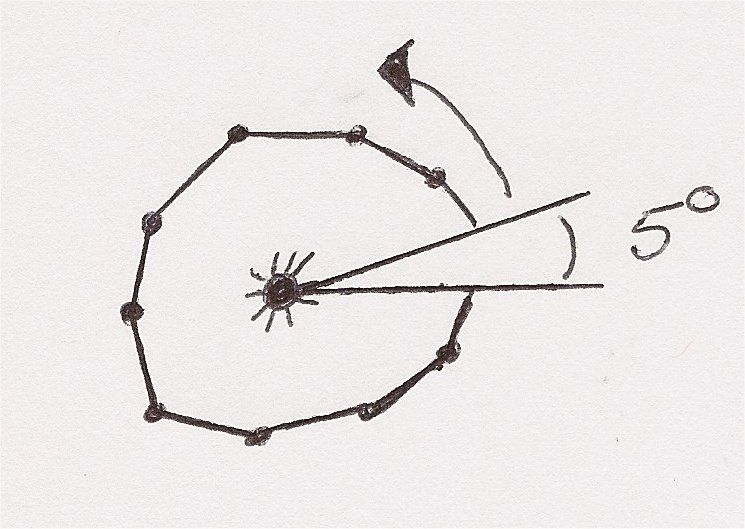
\includegraphics[width=0.5\textwidth]{Figure31.jpg}
%    
\includegraphics[width=0.5\textwidth]{Figure31_gray.jpg}
  \caption{The light source (star) is facing the reader (ie. direction/normal pointing out of the paper.}
	\label{fig:3.1}
\end{figure}

\paragraph{}
Next, the VPL's will be structured at every 5 degrees around the z-axis of the light source resulting in 90degrees/5degrees per ray = 18 rays of VPL's for every one of the 72 rays around the y-axis.  This totals in 1296 rays plus the vertical ray along the y-axis resulting in 1297 rays to form a hemisphere around the light. See figures \ref{fig:3.2} and \ref{fig:3.3}.

\begin{figure}[h!]
  \centering
    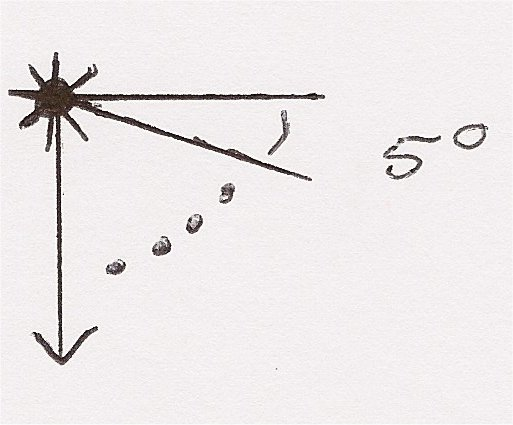
\includegraphics[width=0.5\textwidth]{Figure32.jpg}
%    
\includegraphics[width=0.5\textwidth]{Figure32_gray.jpg}
  \caption{The light source (star) is facing downwards. Angles are drawn to scale.}
	\label{fig:3.2}
\end{figure}


\begin{figure}[h!]
  \centering
    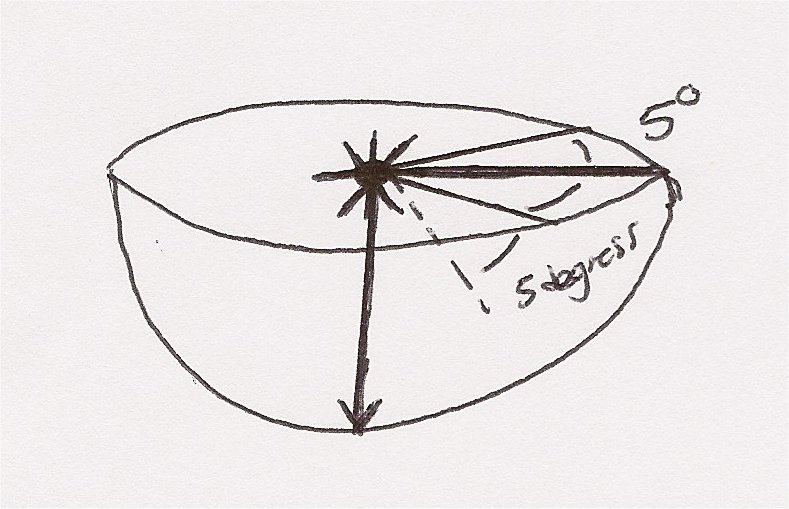
\includegraphics[width=0.5\textwidth]{Figure33.jpg}
%    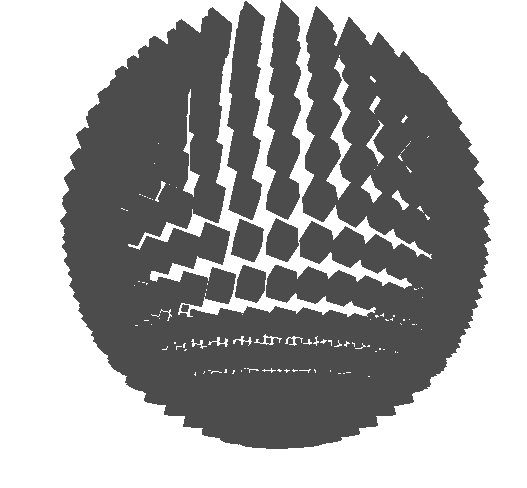
\includegraphics[width=0.5\textwidth]{Figure33_gray.jpg}
  \caption{Figures \ref{fig:3.1} and \ref{fig:3.2} together form a hemisphere. View is looking slightly up at the hemisphere.}
	\label{fig:3.3}
\end{figure}

\paragraph{}
Next, we will have multiple VPL's on each of these rays.  This implementation will have 5 VPL's per ray.  This results in having 5 stacked hemispheres of increasing radii and a total of 6485 VPL's. See figure \ref{fig:3.4}.

\begin{figure}[h!]
  \centering
    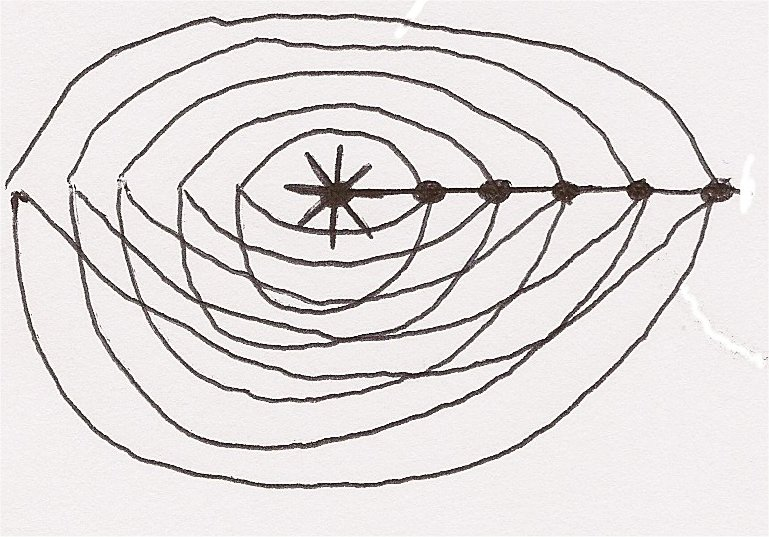
\includegraphics[width=0.5\textwidth]{Figure34.jpg}
%    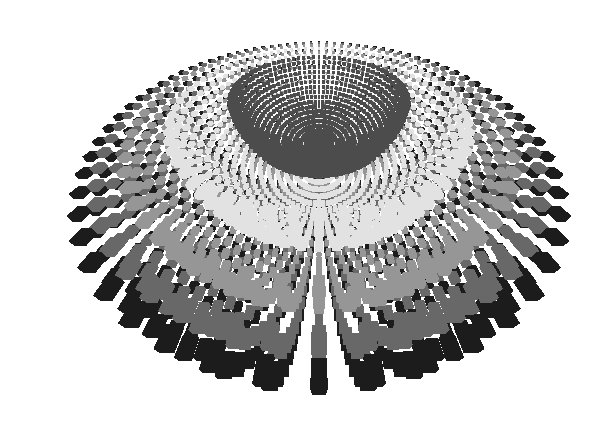
\includegraphics[width=0.5\textwidth]{Figure34_gray.jpg}
  \caption{5 stacked hemispheres formed by the VPL's around the primary light source. Each hemisphere is a different shade to make distinguishing easier.}
	\label{fig:3.4}
\end{figure}

\paragraph{}
The distance from the primary light to each of the VPL's on each ray will be calculated based off of the depth of the scene.  The distance between VPL's on each ray will be logarithmic as shown below and the attenuation will be exponential.  See figure \ref{fig:3.5}.

\begin{figure}[h!]
  \centering
    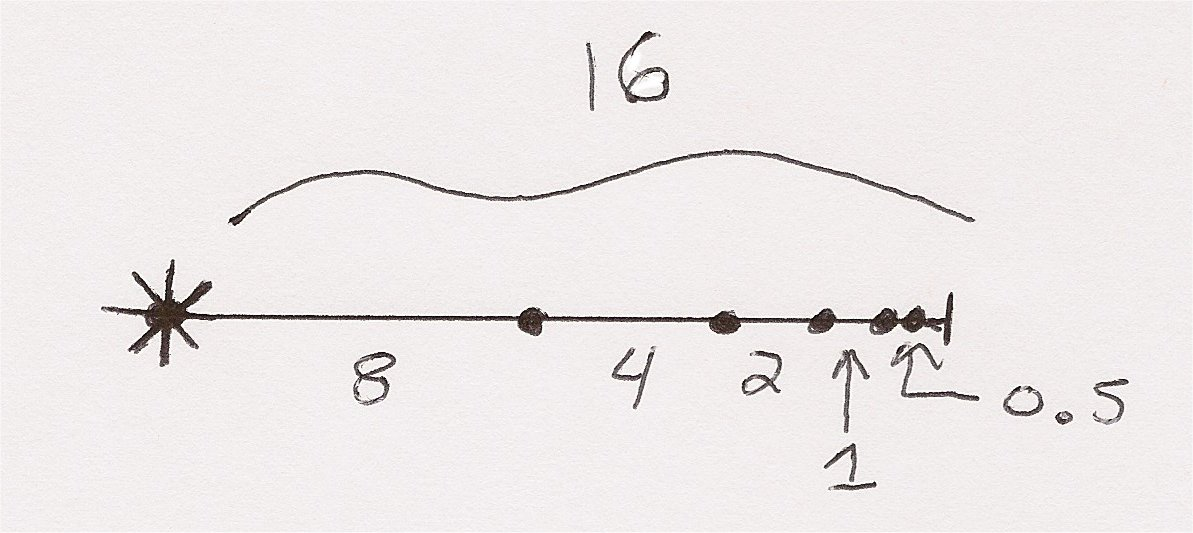
\includegraphics[width=0.5\textwidth]{Figure35.jpg}
%    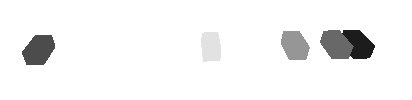
\includegraphics[width=0.5\textwidth]{Figure35_gray.jpg}
  \caption{Showing the logarithmic distances between the VPL's on each ray.  The first box on the left is the first VPL on the ray with successive VPL's going towards the right. Distance shown to scale. (Light source is not shown)}
	\label{fig:3.5}
\end{figure}

\paragraph{}
The goal of this structure is to simulate multiple waves of VPL's flowing outward from the primary light source in order to simulate the light transport as wave-like and therefore simulate indirect illumination using only the direct illumination of these VPL's while ignoring the bouncing of light among surfaces.  An additional goal of this implementation is to have the resulting technique be scalable.  This organization of the VPL's will allow us to use more or less VPL's depending on quality and performance desires.  As such, we can increase or decrease the corresponding angles to decrease or increase the number of VPL's used as well as increase or decrease the number of hemisphere shells used.  Also, we can use stochastic sampling in order to turn off or on certain VPL's in order to introduce ``noise'' in the implementation as well as decrease the number of VPL's required.  As shown in the previous section, noise can be perceptually pleasing provided it is in smooth graduations.

\paragraph{}
The VPL's contributions will computed as shown in figure \ref{fig:3.6}.  The VPL's will act similar to directional lights in that the normal of the VPL will be used in computing the radiance that it provides.  The major difference, however, is that the VPL will be able to contribute radiance to surfaces that are slightly behind the VPL's normal.  Instead of doting the surface normal with the VPL normal and only allowing for contribution when the dot product is between 0 and 1, we will allow the dot product to be between -0.5 and 1.  This will mean that the VPL's viewable range is 240 degrees instead of 180 degrees.  This further depicts each VPL as wave-like.  The calculation to account for the expanded dot product range will be discussed along with the code explanations of chapter 4.  See figure \ref{fig:3.6}.

\begin{figure}[h!]
  \centering
    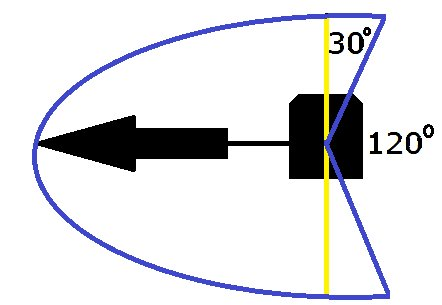
\includegraphics[width=0.5\textwidth]{Figure36.jpg}
%    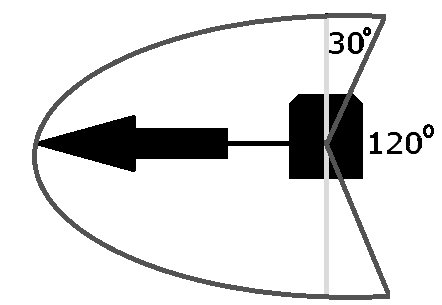
\includegraphics[width=0.5\textwidth]{Figure36_gray.jpg}
  \caption{Showing the wave-like radiance contribution of a VPL. We add an additional 30 degrees of viewable range on the top and bottom limiting the blind spot of the VPL to 120 degrees rather than 180. The arrow signifies the VPL's direction/normal.}
	\label{fig:3.6}
\end{figure}

\paragraph{}
Each VPL normal is calculated using the angles required to rotate the primary light source's direction to point to that specific VPL.  Figure \ref{fig:vplNormals} shows the normals of every VPL.  The resulting shape is a hemisphere of radius 1 due to the normals being normalized.  It also shows that the VPL normals point outward in all negative-y directions from the primary light source.

\begin{figure}[h!]
  \centering
    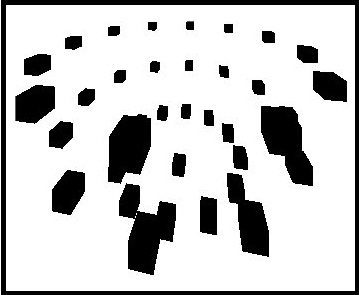
\includegraphics[width=0.5\textwidth]{vplNormals.jpg}
  	\caption{Showing the normals of every VPL. Using ray angle of 30 degrees to simplify the graphic.}
	\label{fig:vplNormals}
\end{figure}

\paragraph{}
Lastly, occlusion will be handled with a shadow map as in \cite{Williams1978} and \cite{Reeves1987} to render shadows for the direct illumination based solely off of the primary light source.  This method is very cheap and provides sufficient shadows for the purposes of this implementation.  This implementation will try two different techniques of rendering indirect shadows.  The first technique will handle indirect occlusion through the use of regular shadow maps on 20 randomly sampled VPL's and will render shadows solely on the information gathered in the 20 shadow maps meaning that we will have 1 direct shadow and 20 indirect shadows.  Therefore, these shadows are computed using accurate visibility and this method will be referred to as ``accurate shadows.''  See figure \ref{fig:20randomVPLs}.  The second technique will handle indirect occlusion through the use of regular shadow maps rendered using 5 specific VPL's and will render shadows by integrating between each of the 5 shadow maps.  The VPL's are equidistant from one another and provide maximum coverage of the scene.  See figure \ref{fig:5specificVPLs}.  By doing this, we will require less shadow maps but will render more indirect shadows.  All of the shadows except for the 5 shadows that come directly from the shadow maps do not use accurate visibility.  Instead, these shadows come from the act of integrating or interpolating between each of the 5 shadow maps and so this method will be referred to as ``integrated shadows.''  The specific implementation details for both techniques will be discussed in chapter 4 with code excerpts present.

\begin{figure}[h!]
  \centering
    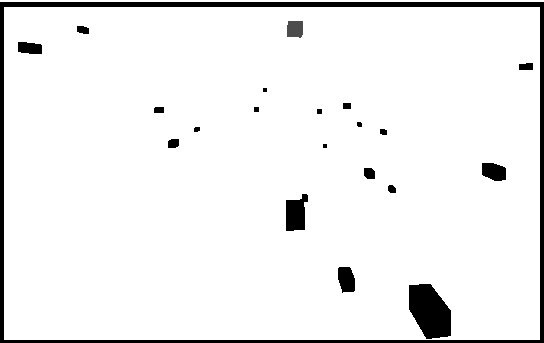
\includegraphics[width=0.5\textwidth]{20randomVPLs.jpg}
  	\caption{Showing 20 randomly sampled VPL's with the primary light source at the top center of the image.}
	\label{fig:20randomVPLs}
\end{figure}

\begin{figure}[h!]
  \centering
    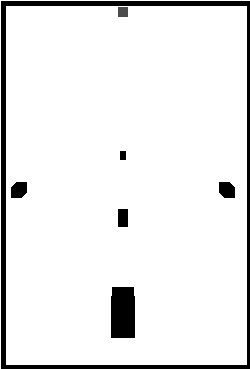
\includegraphics[width=0.5\textwidth]{5specificVPLs.jpg}
  	\caption{Showing 5 specifically chosen VPL's with the primary light source at the top center of the image.}
	\label{fig:5specificVPLs}
\end{figure}

\subsection{GPU AND CPU FUNCTIONS}
\paragraph{}
This implementation will be designed to use both the CPU and the GPU.  The CPU will handle all preliminary tasks such as setting up the window, initializing variables and the shaders, setting up the scene including positioning the light source and objects, handling interactive actions including keyboard callbacks, initializing and filling textures, and initializing the VPL's position, direction, and attenuation.  The CPU will compute all of the necessary VPL data and store it in textures to be passed to the GPU to be used later in the lighting calculations.  This action will need to be performed every time the light is moved.  The CPU will also be used to generate the shadow maps for the direct and indirect shadows by rendering the scene from each of the chosen light's view.  This action will need to be done every time an object or the light is moved.

\paragraph{}
The GPU will calculate shading and illumination for the vertices inputted using the VPL data texture and will calculate shadows based off of the provided shadow maps passed in from the CPU.  Using the GPU to perform these actions are desired due to the GPU's ability to excel in parallel processing of data.  Since the same calculations are performed for every vertex in the scene, each vertex illumination can be calculated in parallel in no specific order allowing these calculations to be performed faster than on the CPU.  These calculations are programmed using GLSL which will be discussed shortly.

\subsection{OPENGL}
\paragraph{}
OpenGL or Open Graphics Library is a multi-platform API for graphics that will be used for this implementation.  The technique is being designed on a machine with OpenGL 4.2.0, however, OpenGL 2.1 and above will be supported.  Also, the technique will run on both Windows and Macintosh.

\subsection{GLSL}
\paragraph{}
GLSL or OpenGL Shading Language is a high-level C-syntax shading language to be used with OpenGL in order to give the developer control over what instructions are executed in the vertex and fragment shaders of the graphics pipeline.  In this implementation, all illumination and shading calculations are computed in the vertex and fragment shaders programmed manually through the use of GLSL.  The technique is being designed on a machine with GLSL 4.20 support, but the shaders are written with GLSL 1.20 support.

\subsection{WORKING ENVIRONMENT}
\paragraph{}
The implementation is being designed and tested on the following hardware and software using the following libraries.  Any and all results such as rendered images and fps results will be gathered while running the method on the following.
\vspace{5 mm}

\textbf{HARDWARE}
\begin{itemize}
\item CPU: AMD Athlon 64 X2 Dual Core 5200+ 2.61Ghz
\item GPU: Nvidia GeForce GTX 465 (1GB memory)
\item Memory: 6.00GB
\end{itemize}

All other hardware specifications are irrelevant.
\vspace{5 mm}

\textbf{SOFTWARE}
\begin{itemize}
\item OS: Windows 7 64-Bit
\item Languages: C++, OpenGL 4.2.0 (2.1 tested/supported), OpenGL Shading Language 4.20 (written using version 1.20)
\item Developer Tools: Microsoft Visual Studio 2008
\end{itemize}
\vspace{5 mm}

\textbf{LIBRARIES}

\vspace{1 mm}

The following libraries are used in this implementation:

\begin{itemize}
\item OpenGL Easy Extension Library (GLEE)
\item OpenGL Extension Wrangler Library (GLEW)
\item OpenGL Utility Toolkit (GLUT)
\end{itemize}

